%
% 1. process this file with pdflatex
% 2. remind to process it twice otherwise cross-references will be wrong
%
\documentclass[a4paper,12pt]{article}
%
% This is to create hyperlinks for index, URLs and citations
% (now we can use the command \url{...} to create URL with hyperlink)
% 
\usepackage{color}
\usepackage[a4paper,colorlinks=true,urlcolor=blue,citecolor=blue,linkcolor=blue,bookmarks=false]{hyperref}
%
% This allows inclusion of pictures.
% Create figures with PowerPoint and then export them individually
% in PDF, PNG, JPEG, or GIF format (in order of preference)
%
\usepackage[pdftex]{graphicx}
\DeclareGraphicsExtensions{.pdf,.png,.jpg,.gif}
%
% Definition of margins
%
\usepackage[top=2cm,bottom=2cm,left=2cm,right=2cm]{geometry}
%
% Paragraph skip and indent
%
\setlength\parskip{\medskipamount}
\setlength\parindent{0pt}
%
% Frequently used abbreviations.
% Note that if there is a space after an abbreviation then it must be quoted:
%-  example1: \ie\ this is an example
% - example2: the \ipsec\ protocol
% but tehre is no need for this when there is a punctuation mark
% - example3 (note the full stop at the end): we use SSL rather than \ipsec.
%
\def\eg{e.g.}
\def\ie{i.e.}
\def\ipsec{IPsec}
\def\myfig#1{Fig.~#1}
\def\mytab#1{Tab.~#1}
\def\rfc#1{RFC-#1}% usage: \rfc{1422}
\def\baseline{Baseline Pseudonyms}
\def\hybrid{Hybrid Scheme}
%
\begin{document}

\title{Vanet Simulator
\\
{\normalsize Report for the Computer Security exam at the Politecnico di Torino}
}
\author{Walter Dal Mut (161600)\\Armand Sofack (124515)
\\
{\normalsize tutor: Giorgio Calandriello}
}
\date{June 2009}
\maketitle

\vfill

\rule{\textwidth}{1pt}

\tableofcontents

\rule{\textwidth}{1pt}

\vfill

\newpage
\section{Introduction}
\section{UML Diagrams}
\section{Security Implementations}
\subsection{\baseline}
\subsection{Security Implementations}
\subsubsection{\baseline}
For the $i$-th pseudonym the CA provide a valid certificate with the public key signed by the CA and a private key for signing messages.\\
The easy way for realize this security implementation is to attach after every message a digital signature and the certificate used for signing message. In this way a vehicle which receive the message can verify the validity of certificate and so verify the digital signature of message. It's really important that pseudonyms is used only for a few time $\tau$ for provide security against the track message reception, because if I use the same certificate for a long period of time an attacker can follow the certificate and identify the car which send messages. This implementation it's really difficult to implement because the message is too long because if we sum the message length plus the signature plus certificate with public key we have a big packet to send on network. For resolve the overhead problem we can use three optimizations \cite{calandriello}.\\Certificate and identify the car which send messages. This implementation it's really difficult to implement because the message is too long because if we sum the message length plus the signature plus certificate with public key we have a big packet to send on network. For resolve the overhead problem we can use three optimizations \cite{calandriello}.\\
The main problem of \baseline is based on certificate because this implementation use a preset of certificates, around a thousand, for sign beacons and send on network. For privacy reasons we can not re-use certificates and after a period of time, for that the life-time of \baseline is dependently from certificate preloaded and this is a real problem because we have to insert new certificates after a period of time and for users that could really invasive.
\subsection{\hybrid}
\section{Simulation Framework implementation}
\section{Implementation, Simulations and Tests}
VANET Simulator is written in Java because this programming language is really powerful and flexible to use but more over we see the Java problems with cryptography. First of all the Java security implementation, at this time (version 1.6.x), do not include elliptic curves for asymmetric cryptography and we have been able to find  on Internet a provider which release elliptic curves : found \textit{Bouncy Castle}\footnote{See bibliography at \pageref{bibliography} for more details on this provider}, then we decided to  use 163 bits  of security level of digital signature \textit{nistb}, after that we have also computed with \emph{openssl}\footnote{See bibliography at page \pageref{bibliography} for more details} the typical speed\footnote{For computation we have used: Pentium 4 Core 2 Duo, processor: Intel T5450 (1.66GHz, 667 Mhz FSB, 2 MB L2 Cache, 2 GB DDR2 RAM} for sign and verify a digital message, see table \ref{tab:OpensslVelocity} at page \pageref{tab:OpensslVelocity}.
\begin{table}[!ht]
	\centering
	\caption{OpenSSL Speed Analysis}
	\begin{tabular}{|c|c|c|c|c|}
	\hline\hline 
	\textbf{Provider} & \textbf{Sign} & \textbf{Verify} & \textbf{sign/s} & \textbf{verify/s} \\
	\hline
	OpenSSL & 0.0017s & 0.0050s & 583.5 & 199.3 \\
	\hline
	Bouncy Castle & 0.028031s & 0.017342s & 35.6 & 57.6 \\
	\hline
	\hline     %inserts single line 
 	\end{tabular} 
	\label{tab:OpensslVelocity}
\end{table}
The Bouncy Castle implementation is slowly than OpenSLL and we have found a difference time order  between C (OpenSSL)  implementation and Java implementation (Bouncy Castle), see table \ref{tab:OpensslVelocity} at page 
After additional analysis we verified the certificates with the certification authority and for doing that in Java it last typically $0.038708s$ roughly $25.83 {verify \over s}$
\subsection{Real Vanet implementation to Simulator}
The main task of Vehicular Networks is privacy, integrity and not repudiation of messages and for do that we use a lot of methods, like pseudonyms change or group keys. In the simulator we are obliged to use all network stack from application level to physical level and this feature remove privacy because we are not able to change MAC address dynamically and if we analyze the network traffic we can found MAC address and track vehicle moves. Real system do not use the complete network stack and work only on level two (MAC layer) with changing MAC address for every beacon sent on the network.
\subsection{Simulation of Baseline Pseudonyms}
Before starting simulation in baseline pseudonyms you have to modify the configuration file \textit{base.properties} \footnote{See the user manual for more information around configurations. Section \ref{usermanual:baseconfiguration} at page \pageref{usermanual:baseconfiguration}} under folder \textit{properties} in root directory of VANET Simulator.\\
For \baseline we can realize three different optimizations picked up from \cite{calandriello} but in this simulator we have implemented the second optimization, in particular the sender append \textit{beacon identification}, \textit{signature}, \textit{public key} and \textit{certificate} only for $\alpha$ messages and transmit only \textit{beacon identification} and \textit{signature} for remaining $\alpha-1$ beacons. \\
The beacon identification is random number compute on four byte without consider other vehicles, is reasonable to use this method without remember other IDs is because probability which two vehicle use the same identification number is really small.
\baseline use optimization two from \cite{calandriello} for limit cryptography overhead, see section \ref{sec:CryptographyOverhead} at page \pageref{sec:CryptographyOverhead} for importance of cryptography overhead, and you can change parameters for realize you personal optimization, for example certificate reattach after tot beacons and certificate or change certificate after a period of time.
\subsection{Performance of Simulator}
For analyze performance of Simulator (figure \ref{fig:performance} at page \pageref{fig:performance}) we have computed statistics for understand the number of signature which we are able to do with the simulator. We have set up the \baseline simulator and set logger into console, after that we have ran system and observed behaviors after changing  the number of beacons/sec and the number of vehicles into wireless area.
\begin{figure}[ht]
% If the picture uses fonts of the correct size (10 ... 12 pt)
% then can be included without scaling
%\centerline{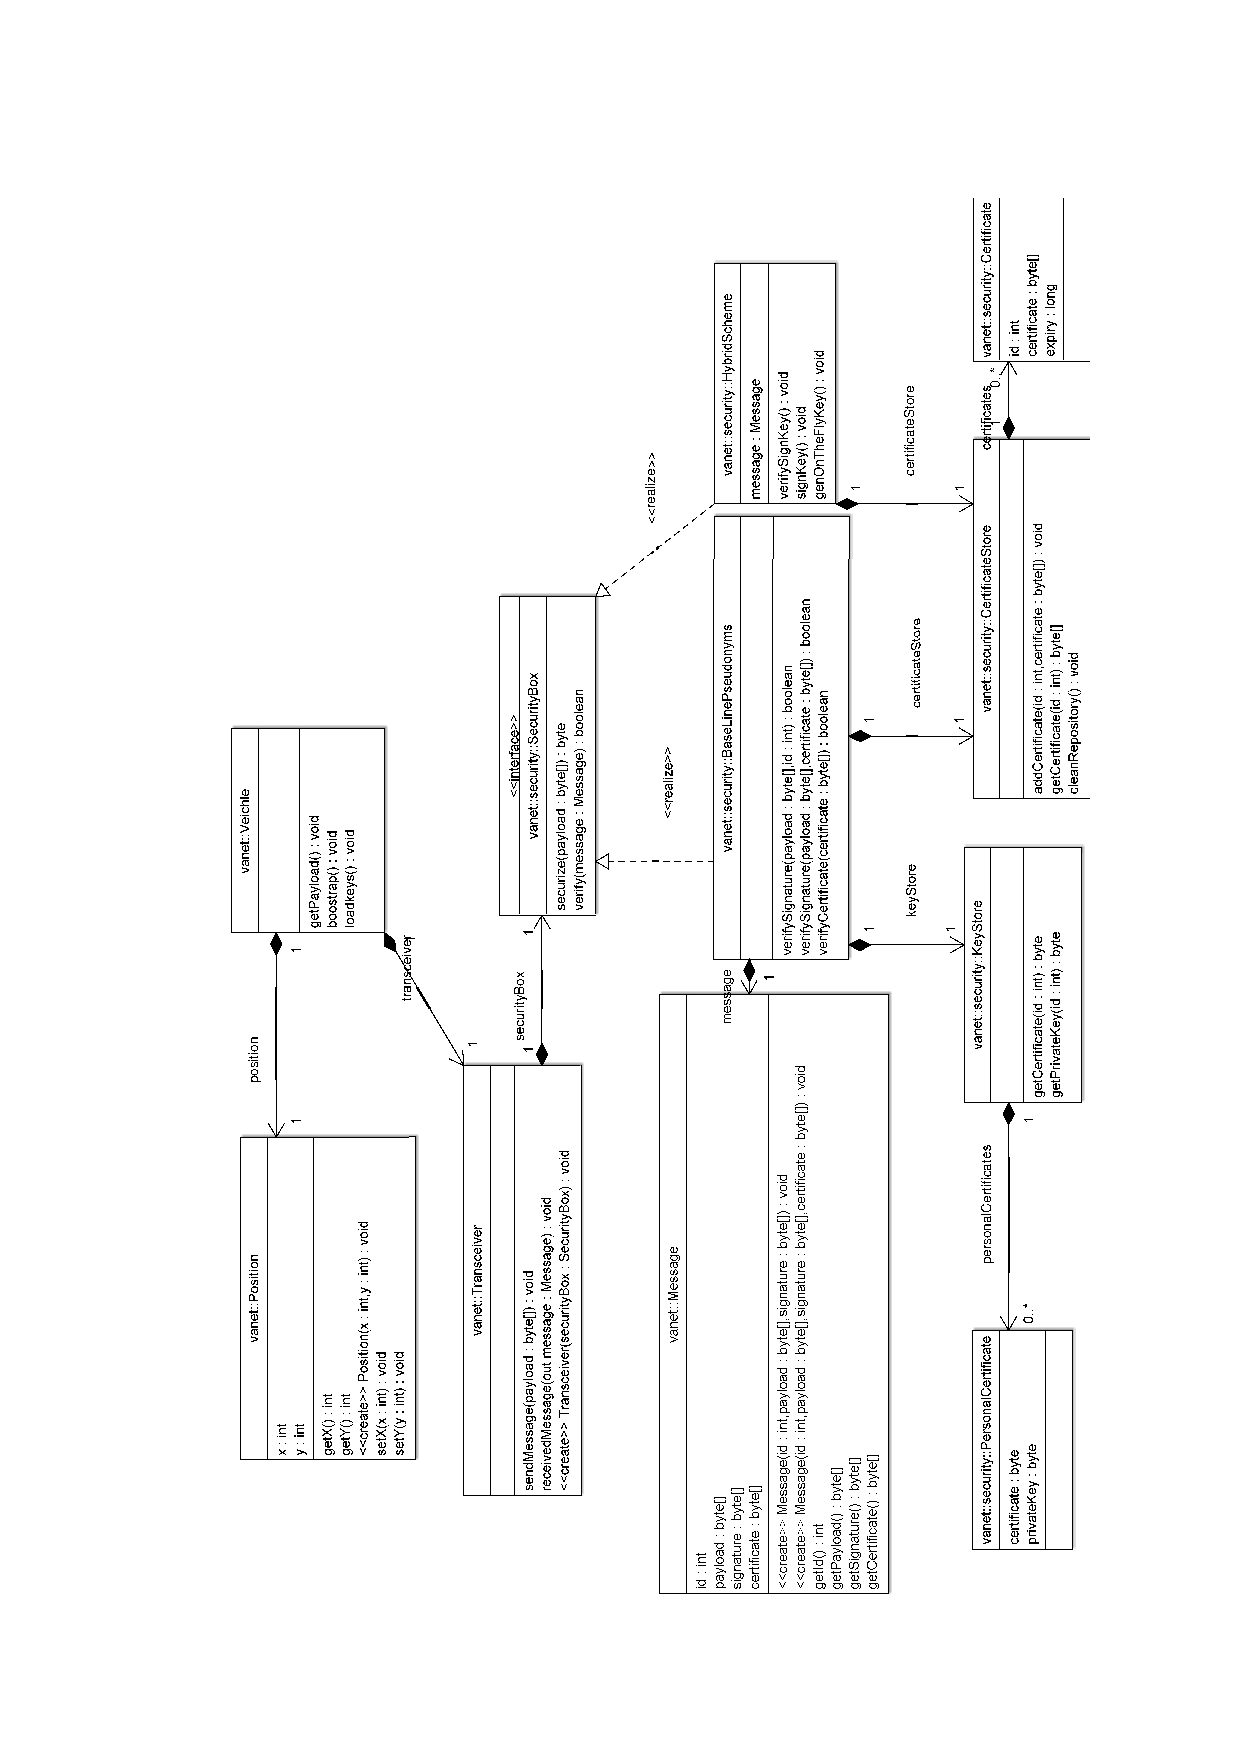
\includegraphics{class_diagram.pdf}}
% otherwise see the example in the following (commented out) line
% to scale it relatively to the page width
\centerline{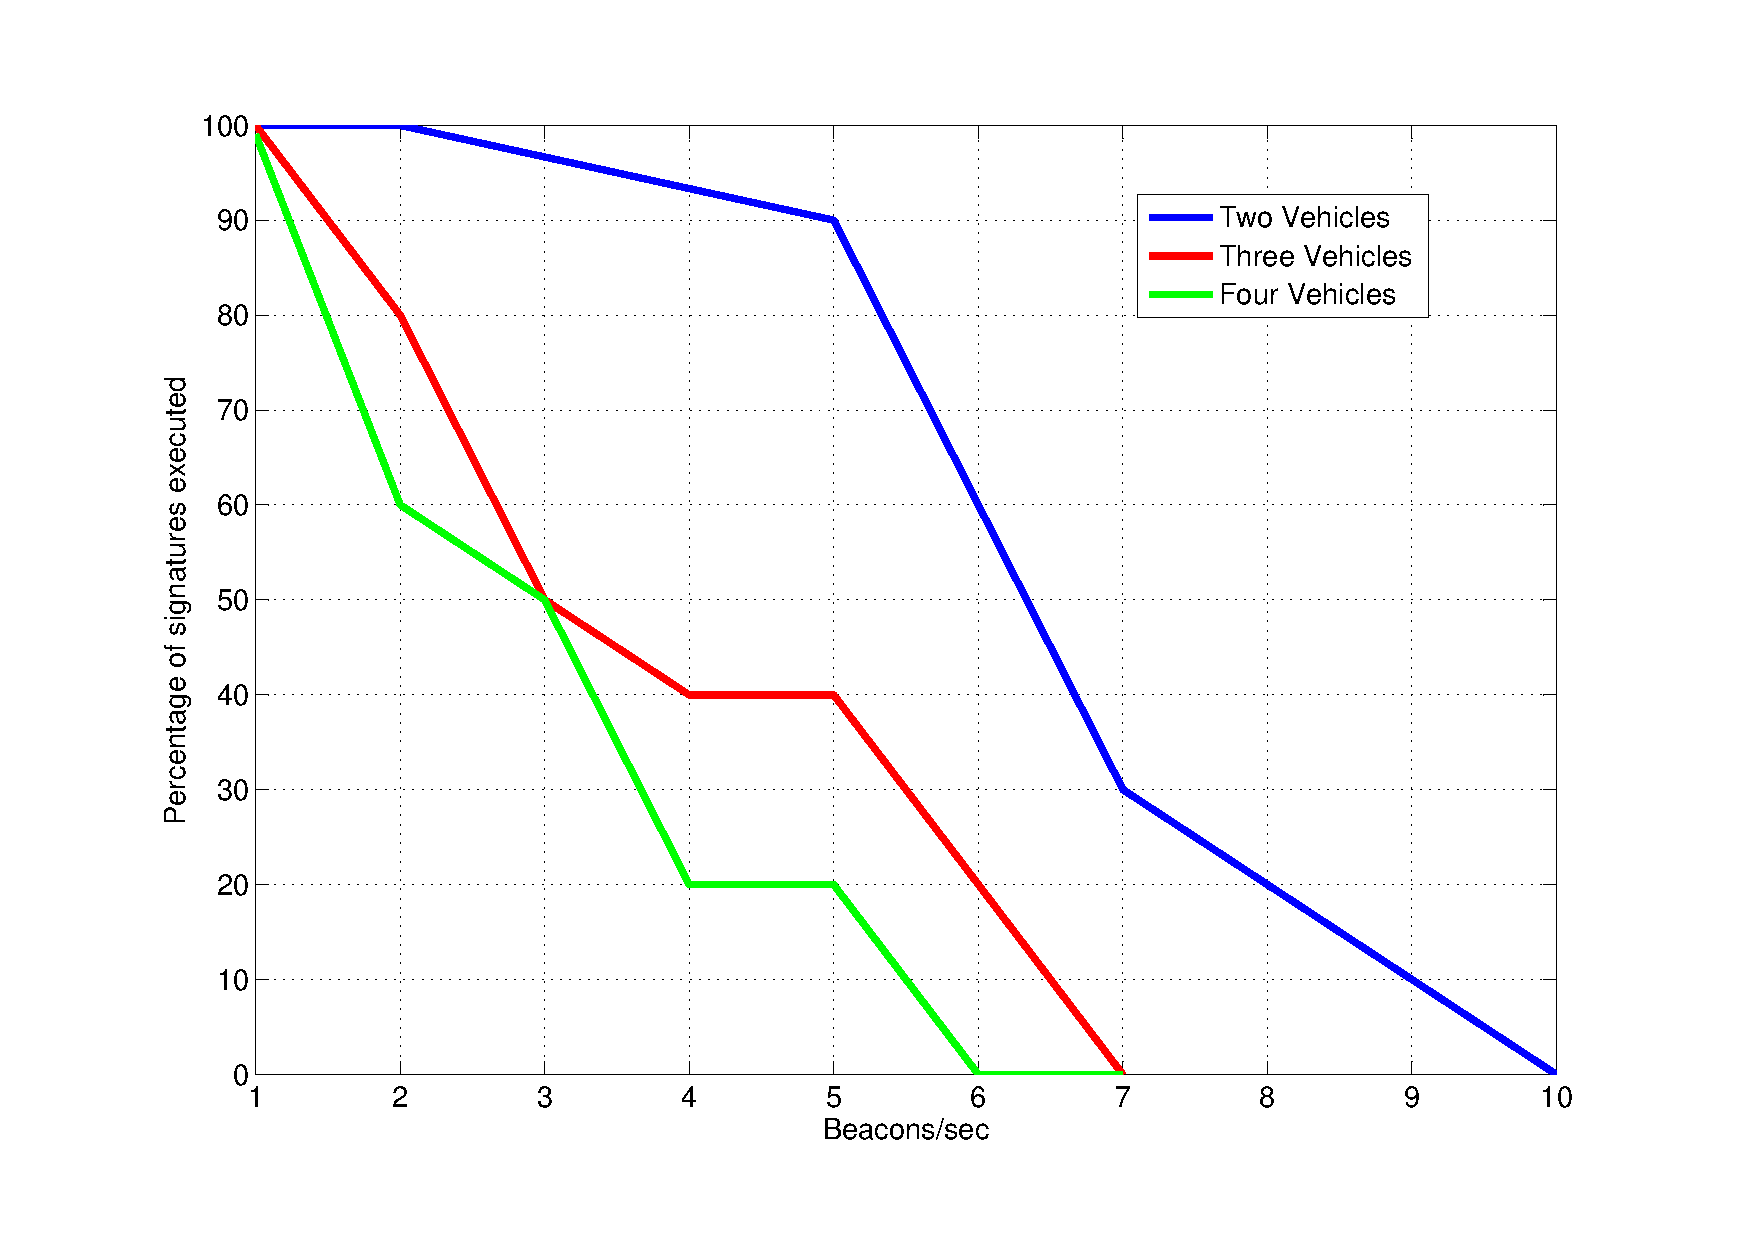
\includegraphics[width=0.8\textwidth]{chart_baseline.pdf}}
\caption{Performance of simulator}
\label{fig:performance}
\end{figure}
\section{Test and profile of simulations}
\section{Comparisons and conclusions}
\section{Documentation}
\subsection{User Manual}
In this part of this monography we explain the possibilities offred by configurations for using the Vanet Simulator in all of it parts. In particoular the main features offered by simulator are changing the security implementation passing by \baseline and \hybrid implementations and configure vehicles on the road, the number of beacons sent during the simulations and modifing logging system for understanding results of simulation.\\
The Vanet Simulator is completly configurable modifing it\'s configurations files under the folder \textit{properties} in the root directoty of simulator.
\section{Documentation}
\subsection{User Manual}
In this part of monograph y we explain the possibilities offered by configurations for using the Vanet Simulator in all of it parts. In particular the main features offered by simulator are changing the security implementation passing by \baseline and \hybrid implementations and configure vehicles on the road, the number of beacons sent during the simulations and modifying logging system for understanding results of simulation.\\
The Vanet Simulator is completely configurable modifying it's configurations files under the folder \textit{properties} in the root directory of simulator.
\subsubsection{Base Configurations}\label{usermanual:baseconfiguration}
The base configurations provide modifications in the core of Vanet Simulator, in particular you can change the \textit{base.properties} file for change core properties like beacons sent, security implementations and others base properties.
If you open the configuration file you see:
\begin{verbatim}
#Max speed in km/h
max_speed = 140
#Max 802.11 cover in meters
wifi_cover = 200
#Access Point broadcast point
server_broadcast_point = 127.255.255.255
#Server Port
server_port = 55055
#Beacons/sec
beacons_sec = 0.1
#If you want no moves of vehicles
no_moves = true
#choose simulator BP or GS
simulator = bp
#max certificate validity into area in seconds
maxCertificateValidityTime = 33
#Reattach certificate every tot beacons
reattachCertificate = 5
#MYSQL properties
mysql_host=127.0.0.1
mysql_username=root
mysql_password=
mysql_database=vanet
#Define the log system
#  0 MYSQL log
#  1 File log
#  2 StdOut log
logSystem=0
\end{verbatim}
For detailed information you can see table \ref{tab:BaseConfiguration} at page \pageref{tab:BaseConfiguration}.
\begin{table}[!ht]
	\centering
	\caption{Base Configuration specifications}
	\begin{tabular}{|c|c|c|}
	\hline\hline 
	\textbf{Property Name} & \textbf{Property Translation} & \textbf{Property Type} \\
	\hline
	max\_speed & The maximum speed of vehicles & int \\
	\hline
	wifi\_cover & The maximum wireless area coverage & int \\
	\hline
	server\_broadcast\_point & The broadcast node for send messages & string \\
	\hline
	server\_port & The port for receive messages & int \\
	\hline
	beacons\_sec & The number of beacons sent in one second & float \\
	\hline
	no\_moves & Lock vehicles into the map & boolean \\
	\hline
	simulator & The simulator which you want use. & string\\
	{} & BP for baseline implementations. & {} \\
	{} & GS for group signature implementation & {} \\
	\hline
	maxCertificateValidityTime & The maximum time for certificate validity & int \\
	\hline
	reattachCertificate & Reattach the certificate every tot beacons & int \\
	\hline
	mysql\_host & The host for mysql & string \\
	\hline
	mysql\_username & Username for authenticate into mysql & string \\
	\hline
	mysql\_password & Password for authenticate into mysql & string \\
	\hline
	mysql\_database & Database to use & string \\
	\hline
	logSystem & The log system which you want use. & int\\
	{} & 0 for mysql log system. & {} \\
	{} & 1 for log data into a files & {} \\
	{} & 2 for log data on console & {} \\
	\hline
	\hline     %inserts single line 
 	\end{tabular} 
	\label{tab:BaseConfiguration}
\end{table}
\subsubsection{Vehicle Configurations}\label{usermanual:vehicleconfigurations}
The vehicles configurations set the status of roads into the simulator. In particular you can modify the number of vehicles into the road, velocity and initial position.\\
The configuration file for vehicle is XML (eXtensible Markup Language) based and is named \textit{vehicles.xml} and positioned into folder \textit{vehicles}; if you open this file you see:
\begin{verbatim}
<?xml version="1.0" encoding="UTF-8"?>
<Vehicles>
    <Vehicle id="1" speed="100" x="10" y="20" />
    <Vehicle id="2" speed="120" x="20" y="50" />
</Vehicles>
\end{verbatim}
Every tag, excluding root tag, identify a new vehicle with attributes like options, in particular you can modify the vehicle identification number changing the \textit{id} attribute or you can change the vehicle speed modifying the \textit{speed} attribute or the position of the vehicle using the \textit{x} or \textit{y} attributes.
For the \baseline~operating mode you have to link certificates and private keys to each vehicles, for doing that you have to follow instruction in section \ref{usermanual:preloadkey} at page \pageref{usermanual:preloadkey}
\subsubsection{Why many log configurations}
The log system for this application is really difficult, in fact the normal std out or file log system is too slow and produce conflicts if you send a lot of beacons during sign and verify operation but it's really useful because you can understand immediately what the system are doing in real time, the other methods are a middle solution for see result and velocity during sign and verify and the best solution for velocity but difficult to understand in real time the system but it's useful for post-processing. For this reason we have written three type of log system for use the best method when that are compatible with the simulation.
\subsubsection{Log configuration}\label{usermanual:logconfiguration}
The log system use the \textit{log4j} module for write sensible information of simulator. The system provide three log configurations, on standard output stream, file stream or on MySQL database.\\
The configuration of log system it's really powerful and you can set the level of logging or change the log representation for standard out stream or file stream. The configuration of log system is divided into three file, ones for each method and it's collected into folder \textit{properties} which names \textit{stdout.properties} for standard out, \textit{file.properties} for file stream or \textit{mysql.properties} for MySQL database log system.
\subsubsection{MySQL database configuration}
For using MySQL database log system you have to configure the database before launching the Vanet Simulator. You have to create or import a database with tables definition into MySQL using the \textit{vanet.sql} file under the \textit{properties} directory.\\
For import the database and tables definition you have to enter in you MySQL command line and create a new database using command:
\begin{verbatim}
mysql> CREATE DATABASE vanet;
\end{verbatim}
After this step you have to create a table in the new database using commands:
\begin{verbatim}
mysql> use vanet;
...
mysql>CREATE TABLE IF NOT EXISTS `logs` (
  `log_id` int(11) unsigned zerofill NOT NULL auto_increment,
  `level` varchar(255) NOT NULL,
  `class_name` varchar(255) NOT NULL,
  `method_name` varchar(255) NOT NULL,
  `message` text NOT NULL,
  PRIMARY KEY  (`log_id`),
  KEY `level` (`level`)
) ENGINE=InnoDB DEFAULT CHARSET=latin1 AUTO_INCREMENT=1 ;
...
\end{verbatim}
After this step you have configured the MySQL database for record logs from Vanet Simulator.
\subsubsection{Install Vanet Simulator on Windows}
For install Vanet simulator on Windows operating system you can use the installer \textit{setupVanetSimulator.exe} and follow the screen information for complete the setup of application.\\
After install procedure you have to open a new console and go into install directory and send the command
\begin{verbatim}
C:\Program File\Vanet Simulator\>java -jar vanetSimulator.jar
\end{verbatim}
After this command you see the bootstrap procedure and after the system run. The default log operation is the standard out and you can see directly all the informations.\\
The common output on screen are this:
\begin{verbatim}
.:: Bootstrap ::.
Loading base properties
Base properties loaded
Loading vehicles configuration
security/certificates/1/c
security/certificates/2/c
Vehicles configuration loaded
.:: Bootstrap end ::.
\end{verbatim}
\subsubsection{Install Vanet Simulator on generic OS}
For install Vanet Simulator you have to setup all folders and executable jar manually. Create new folder in a point of file system and enter in it, after that copy the content of \textit{build} directory and now you can send the command for start the simulator.
\begin{verbatim}
name@domain$ java -jar vanetSimulator.jar
\end{verbatim}
After this command you see the bootstrap procedure and after the system run. The default log operation is the standard out and you can see directly all the informations.\\
The common output on screen are this:
\begin{verbatim}
.:: Bootstrap ::.
Loading base properties
Base properties loaded
Loading vehicles configuration
security/certificates/1/c
security/certificates/2/c
Vehicles configuration loaded
.:: Bootstrap end ::.
\end{verbatim}
\subsubsection{Add certificates and private keys for \baseline}\label{usermanual:preloadkey}
When the system doing the bootstrap in \baseline~mode research certificate and private keys for doing digital signatures.\\
Security properties are in \textit{security} folder, if you add one vehicle you must attach certificates and private keys for work with \baseline~implementation. For do that you have to create a set of folders and positioning certificates and keys in a right place. Under \textit{security} you have one folder named \textit{certificates} and under that folder you have another one folder for each vehicle named with the \textit{vehicle id} (section \ref{usermanual:vehicleconfigurations} at page \pageref{usermanual:vehicleconfigurations}), create new folder named with unique integer identification. Under this folder you have to create another two folders named \textit{c} for certificates and \textit{p} for private keys; after this steps you have to copy your private keys in folder \textit{p} and certificates in folder \textit{c}. Certificates and private keys must have the same name for link, for example: \textit{sec1.crt $\rightarrow$ sec1.key}.tificates and keys in a right place. Under \textit{security} you have one folder named \textit{certificates} and under that folder you have another one folder for each vehicle named with the \textit{vehicle id} (section \ref{usermanual:vehicleconfigurations} at page \pageref{usermanual:vehicleconfigurations}), create new folder named with unique integer identification. Under this folder you have to create another two folders named \textit{c} for certificates and \textit{p} for private keys; after this steps you have to copy your private keys in folder \textit{p} and certificates in folder \textit{c}. Certificates and private keys must have the same name for link, for example: \textit{sec1.crt $\rightarrow$ sec1.key}.



\begin{thebibliography}{99}
%
% Citations will be numbered according to the order
% in which they are listed in this section.
%
\bibitem{calandriello}
P.~Papadimitratos, G.~Calandriello, J.-P.~Hubaux, A.~Lioy,
``Efficient and Robust Pseudonymous Authentication in VANET'',
MOVE 2008: IEEE INFOCOM-2008 workshop on Mobile Networking for Vehicular Environments,
Phoenix (AZ, USA), April 13-18, 2008, pp.~19-27 
\bibitem{raya}
P.~Papadimitratos, M.~Raya, J.-P.~Hubaux,
``Securing Vehicular Communications'',
MOVE 2006: IEEE Wireless Communications Intervehicular Communications,
October, 2006, pp.~8-15 
\bibitem{kargl}F.~Kargl, E.~Schoch, B.~Wiedersheim, T.~Leinmuller,
``Secure and Efficient Beaconing for Vehicular Networks'',
VANET 2008: IEEE INFOCOM-2008 workshop on Mobile Networking for Vehicular Environments,
San Francisco (CA, USA), September 15, 2008, pp.~1-2 
\end{thebibliography}
\end{document}
%
% Before delivering your report, don't forget to run a spell checker,
% such as aspell (with a UK-english dictionary)
%
